\pagebreak

\subsection{Test Results}
The results shown here provide the key information obtained from testing. A full report for each test can be found in Appendix \ref{sec:apptestres}.

\subsubsection{Test 28: Pump Operations}
\label{sec:test28result}

It was found that when the power supply was switched on the current went up to 600 mA for less than one second. It then settled to 250 mA. By covering the air intake, simulating air intake from a lower pressure, the current drops to 200 mA. By covering the air output, simulating pushing air into a higher pressure, the current rises to 400 mA.

Therefore the power for each of these conditions is 14.4 W at turn on, 6 W in normal use, 4.8 W when sucking from low pressure, 9.6 W when pushing to high pressure.

\subsubsection{Test 18: Pump Low Pressure}\label{subsection:pumplowpressuretest}

The pump was tested at low pressure using a small vacuum chamber down to \SI{10}{\hecto\pascal}. Flow rates were recorded from \SI{30}{\hecto\pascal}, the expected highest sampling altitude.

 The results can also be seen in Table \ref{tab:pump-low-pressure-result} and Figure \ref{fig:pump-performance}. Note that the results should be considered an approximation due to the lack of equipment such as flow-meters that would have made this test more precise. 

\begin{table}[H]
\centering

\begin{tabular}{|l|l|l|l|l|l}
\cline{1-5}
\textbf{{\small Altitude(km)}}\par & \textbf{{\small Pressure Start(hPa)}}\par & \textbf{{\small Pressure End(hPa)}}\par & \textbf{{\small Time(sec)}}\par & \textbf{{\small Flow Rate(L/min)}}\par &  \\ \cline{1-5}
24 & 30 & 23 & 60 & 3 &  \\ \cline{1-5}
17 & 87 & 80 & 53 & 3.4 &  \\ \cline{1-5}
11 & 220 & 190 & 37 & 4.9 &  \\ \cline{1-5}
\end{tabular}
\caption{Table Showing the Time Taken Until the 3 L Bag Stopped Expanding at Various Different Pressures.}
\label{tab:pump-low-pressure-result}
\end{table}

\raggedbottom

\begin{figure}[H]
    \begin{align*}
        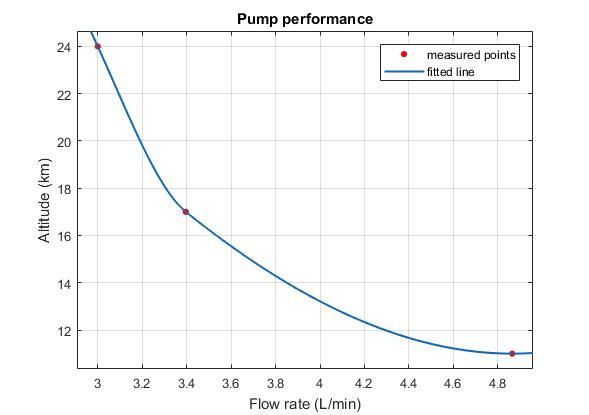
\includegraphics[width=11cm]{5-experiment-verification-and-testing/img/pump-performance.jpg}
    \end{align*}
    \caption {Obtained Pump Performance at Low Pressure.} \label{fig:pump-performance}
\end{figure}

\subsubsection{Test 30: Sampling Bag Bursting}
\label{sec:test30result}

A sampling bag was placed in a small vacuum chamber connected to the pump and the pump was run for 3 minutes with a full bag to see how the bag reacted. 

It was found that there are two potential failure modes. The first is a slow leakage caused by damage to the bag seal and the second is  a rapid failure of the bag seal leading to total loss of the sample.

It can be concluded that, as long as the bags are well secured to the valves at the bottom and through the metal ring at the top, bag bursting during flight would not cause damage to any other components on board. Even during the more energetic burst that occurs from continuous pumping the bag remained fixed to the valve connection and experienced no fragmentation. The consequences of a single bag burst would be limited to loss of data and a disturbance to audio frequencies. 

\subsubsection{Test 29: Pump Current under Low Pressure}
\label{sec:test29result}

In general it was found that decreasing the pressure, or increasing the altitude, lead to a decrease in pump current draw. The full results can be seen in Table \ref{tab:pumpcurrentpressure}. 

\begin{table}[H]
\centering

\begin{tabular}{|l|l|l|l|}
\hline
\textbf{Altitude (km)} & \textbf{Pressure (hPa)} & \textbf{Into Bag Current (mA)} & \textbf{Into Seal Current (mA)} \\ \hline
20 & 57 & 140 & 138 \\ \hline
18 & 68 & 150 & 141 \\ \hline
16 & 100 & 161 & 146 \\ \hline
12 & 190 & 185 & 175 \\ \hline
9 & 300 & - & 200 \\ \hline
6 & 500 & - & 242 \\ \hline
0 & 1013 & - & 218 \\ \hline
\end{tabular}
\caption{Table Showing How the Current Draw of the Pump Changed With Outside Air Pressure for Two Different Conditions. The First Pumping Into a Sampling Bag and the Second Pumping Into a Sealed Tube.}
\label{tab:pumpcurrentpressure}
\end{table}

From the table it can be seen that the current draw is higher during the bag filling than during the sealed case. As the experiment will sample between 11 km and 24 km it can be concluded that the highest current draw will occur during the 11 km altitude sample and can be expected to be around 200 mA. 

\subsubsection{Test 17: Sampling bags' holding times and samples' condensation verification}
\label{sec:test17result}

The main objective of this test was to flush eight 1 L sampling bags with nitrogen, the same way it will be done for the flight. After the flushing is done, fill them with a dry gas and leave them outside for 6, 14, 24 and 48 hours. Then analyze two sampling bags after each time duration and see if the concentration of gases inside has changed. 

After analyzing the sampling bags the obtained results are presented in Figure \ref{fig:test17-results}.

\begin{figure}[H]
    \begin{align*}
        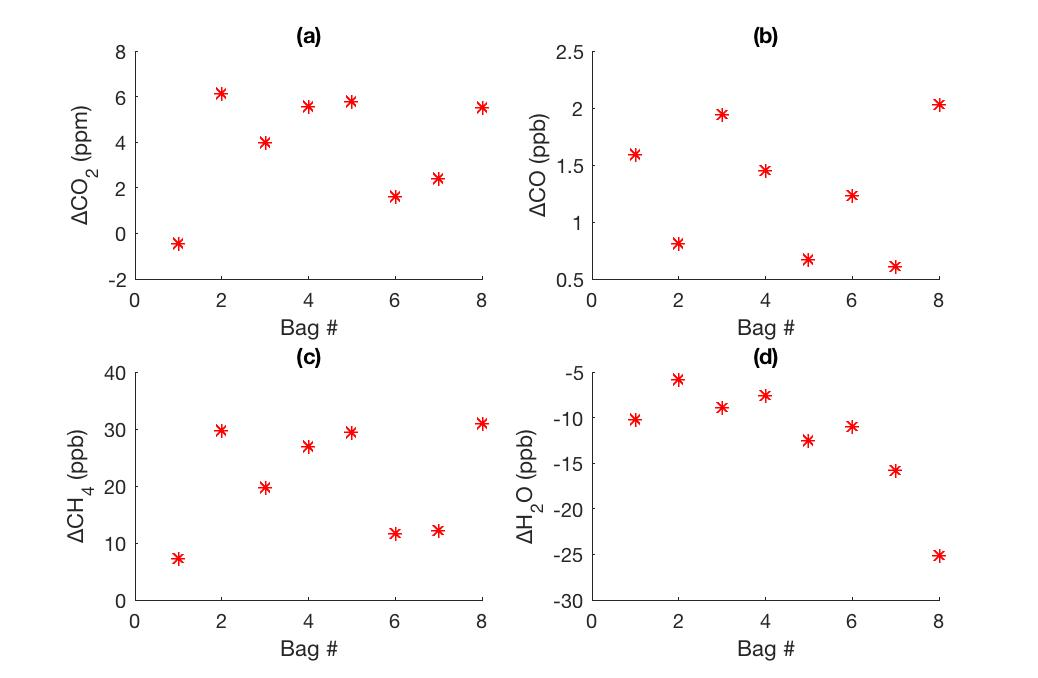
\includegraphics[width=1\linewidth]{5-experiment-verification-and-testing/img/test17-results.jpg}
    \end{align*}
    \caption {Obtained Variation in Concentration for (a) $CO_2$ in ppm, (b) $CO$ in ppb, (c) $CH_4$ in ppb and (d) $H_2O$ in ppb.} \label{fig:test17-results}
\end{figure}


It should be mentioned that the results were not at all what was expected. If the sampling bags held the gases for 48 hours, the analyzed concentration should have been the same as the dry gas used to fill them or the variation should have been smaller. 

A possible explanation for this results could be that the emptying of the sampling bags was not done rigorously enough and that some air/nitrogen was left inside which diluted in the dry gas and changed the concentrations. This effect is even increased due to the smaller size of the used sampling bags (1 L instead of 3 L). This would also explain why the results don't follow any pattern. 

The general outcome of this test is that the team has realized that the flushing of the sampling bags is a very delicate process. This test will be repeated but using the set-up described in Section 4. This test has also been useful to decide that the flushing of the sampling bags should be done with dry gas instead of nitrogen in order to minimize the effects of the nitrogen diluting in the samples. 

% Flushing with nitrogen may alter the results. 

\subsubsection{Test 4: Low Pressure}

The same vacuum chamber was used as in Tests 18 and 29. The Styrofoam was measured on each side before it was placed in the chamber. It was then taken down to 5 hPa and held there for 75 minutes. It was then removed and the sides were measured again. It was found that there was no significant change in dimensions. The results can be seen in Table \ref{tab:styrofoam-test-result}.

\begin{table}[H]
\begin{tabular}{|l|l|l|}
\hline
Side & Before (cm) & After (cm) \\ \hline
A & 9.610 & 9.580 \\ \hline
B & 9.555 & 9.550 \\ \hline
C & 9.560 & 9.565 \\ \hline
D & 9.615 & 9.610 \\ \hline
E & 9.615 & 9.615 \\ \hline
F & 9.555 & 9.550 \\ \hline
G & 9.605 & 9.605 \\ \hline
H & 5.020 & 5.020 \\ \hline
I & 5.025 & 5.025 \\ \hline
J & 5.015 & 5.015 \\ \hline
K & 5.020 & 5.025 \\ \hline
\end{tabular}
\caption{Styrofoam Size Before and After Vacuum.}
\label{tab:styrofoam-test-result}
\end{table}

As some sides are measured slightly bigger after and some slightly smaller it is thought this is due to the measuring technique and not due to changes in the Styrofoam. It is thought the result from side A could be due to deforming the Styrofoam with calipers or a misread original length.

The pump and the airflow sensor were connected together and tested at 16 different pressures. Due to some issues in the data logging with time stamping it is not possible to verify the pump performance until this issue is resolved. A re-test will be made as soon as possible.

\subsubsection{Test 20: Switching Circuit Testing and Verification}

This has begun on breadboards with LEDs replacing the valves until the valves arrive. 
So far DC-DC's have been set up and tested. Sensors have been connected electronically and the next step is to get them to communicate with the Arduino. Mosfets connecting to the pump and the heaters have been tested for switching on and off with good results.

\subsubsection{Test 32: Software Failure}

So far testing has revealed that losing the SD card does not interrupt ground station data, it just means no data will be written to the SD card. However, if you reconnect the SD after removing it currently it will not connect back to the SD card and it as if the SD card has been permanently lost.